\documentclass[tikz,border=2pt]{standalone}
\usepackage{amsmath,amssymb}
\usepackage{tikz}

\begin{document}
% The 3! = 6 orderings of three objects: 3 choices for the first position, 2 for the second,
% 1 for the last.
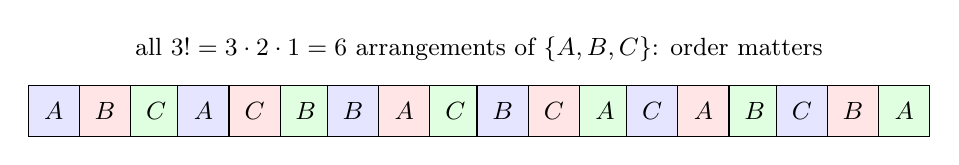
\begin{tikzpicture}[every node/.style={font=\small}]
	\foreach \i/\a/\b/\c in {0/A/B/C, 1/A/C/B, 2/B/A/C, 3/B/C/A, 4/C/A/B, 5/C/B/A} {
		\node[draw, fill=blue!10, minimum size=6.5mm] at (\i*1.9,0) {$\a$};
		\node[draw, fill=red!10, minimum size=6.5mm] at (\i*1.9+0.65,0) {$\b$};
		\node[draw, fill=green!12, minimum size=6.5mm] at (\i*1.9+1.3,0) {$\c$};
	}
	\node[anchor=south] at (5.4,0.5) {all $3!=3\cdot2\cdot1=6$ arrangements of $\{A,B,C\}$: order matters};
	
\end{tikzpicture}
\end{document}
